% Deeper or wider?  A baseline model of where researchers work, and how AI changes it.
% Build:              latexmk -pdf baseline.tex
% Numbers and figure: python3 check_baseline.py   (writes tables/*.tex and figures/mechanism.pdf)
\documentclass[11pt,letterpaper]{article}
\usepackage[T1]{fontenc}
\usepackage[utf8]{inputenc}
\usepackage{mathpazo}
\usepackage{tgpagella}
\usepackage[scale=0.90]{tgheros}
\usepackage[scale=0.92]{tgcursor}
\linespread{1.06}
\usepackage[letterpaper,top=1.1in,bottom=1.15in,left=1.2in,right=1.2in,headheight=15pt,headsep=18pt,footskip=32pt]{geometry}
\usepackage[protrusion=true,expansion=true]{microtype}
\usepackage{amsmath,amssymb,mathtools,bm}
\usepackage[table]{xcolor}
\usepackage{booktabs,tabularx,array}
\usepackage{graphicx}
\usepackage{float}
\usepackage[font=small,labelfont={bf,sf},labelsep=period,skip=6pt]{caption}
\usepackage{enumitem}
\usepackage[most]{tcolorbox}
\usepackage{tikz}
\usetikzlibrary{arrows.meta,positioning,calc}
\usepackage{fancyhdr}
\usepackage{titlesec}
\usepackage{parskip}
\usepackage{needspace}

% ---------------------------------------------------------------- colours
\definecolor{hblue}{HTML}{2A78D6}
\definecolor{hbluedark}{HTML}{104281}
\definecolor{horange}{HTML}{EB6834}
\definecolor{haqua}{HTML}{1BAF7A}
\definecolor{haquadark}{HTML}{0B6B49}
\definecolor{ink}{HTML}{0B0B0B}
\definecolor{inktwo}{HTML}{52514E}
\definecolor{muted}{HTML}{898781}
\definecolor{gridc}{HTML}{E1E0D9}
\definecolor{axisc}{HTML}{C3C2B7}
\definecolor{paperc}{HTML}{F4F3EF}

\usepackage[colorlinks=true,linkcolor=hbluedark,urlcolor=hbluedark,citecolor=hbluedark,
  bookmarksnumbered=true,pdftitle={Deeper or wider? A baseline model},pdfauthor={}]{hyperref}

% ---------------------------------------------------------------- layout
\graphicspath{{figures/}}
\setlist{itemsep=2pt,topsep=3pt,parsep=0pt,leftmargin=1.5em}
\renewcommand{\arraystretch}{1.2}
\newcolumntype{L}{>{\raggedright\arraybackslash}X}
\newcolumntype{P}[1]{>{\raggedright\arraybackslash}p{#1}}
\newcolumntype{C}[1]{>{\centering\arraybackslash}p{#1}}
\setcounter{secnumdepth}{2}
\emergencystretch=1.5em

\titleformat{\section}{\sffamily\bfseries\Large\color{hbluedark}}{\thesection}{0.7em}{}
\titleformat{\subsection}{\sffamily\bfseries\normalsize\color{hbluedark}}{\thesubsection}{0.7em}{}
\titlespacing*{\section}{0pt}{20pt plus 4pt minus 2pt}{6pt}
\titlespacing*{\subsection}{0pt}{12pt plus 3pt minus 2pt}{2pt}

\pagestyle{fancy}
\fancyhf{}
\renewcommand{\sectionmark}[1]{\markright{\thesection\enspace #1}}
\fancyhead[L]{\sffamily\footnotesize\color{muted}Deeper or wider? A baseline model}
\fancyhead[R]{\sffamily\footnotesize\color{muted}\nouppercase{\rightmark}}
\fancyfoot[C]{\sffamily\footnotesize\color{muted}\thepage}
\renewcommand{\headrulewidth}{0.3pt}
\renewcommand{\headrule}{{\color{axisc}\hrule width\headwidth height\headrulewidth}}

% ---------------------------------------------------------------- boxes
\tcbset{hbase/.style={enhanced,breakable,parbox=false,boxrule=0pt,frame hidden,arc=0pt,outer arc=0pt,
  left=11pt,right=10pt,top=7pt,bottom=7pt,before skip=10pt plus 2pt,after skip=10pt plus 2pt,lines before break=4}}
\newtcolorbox{keybox}[1][Key point]{hbase,colback=hblue!6,borderline west={3pt}{0pt}{hblue},
  before upper={{\sffamily\bfseries\small\color{hbluedark}#1}\par\vspace{1pt}}}
\newtcolorbox{notebox}[1][Note]{hbase,colback=paperc,borderline west={3pt}{0pt}{axisc},
  fontupper=\small,before upper={{\sffamily\bfseries\footnotesize\color{inktwo}#1}\par\vspace{1pt}}}
\tcbset{resultstyle/.style={enhanced,breakable,parbox=false,colback=white,colframe=axisc,boxrule=0.5pt,
  arc=1.5pt,left=9pt,right=9pt,top=6pt,bottom=6pt,middle=5pt,lines before break=3,
  before skip=10pt plus 2pt,after skip=10pt plus 2pt,
  colbacktitle=paperc,coltitle=ink,fonttitle=\sffamily\small\bfseries,toptitle=3pt,bottomtitle=3pt,titlerule=0.4pt,
  separator sign={\enspace},description font=\mdseries\color{inktwo},
  fontlower=\small,segmentation style={solid,draw=gridc,line width=0.5pt}}}
\newtcbtheorem{prop}{Proposition}{resultstyle}{prop}
\newtcbtheorem{defn}{Definition}{resultstyle}{def}
\newtcbtheorem[number within=section]{lem}{Lemma}{resultstyle}{lem}
\newcommand{\stepcell}[2]{\parbox[t][0.9in][t]{1.2in}{\raggedright\textbf{#1}\\[3pt]#2}}   % a box of Figure 1
\newcommand{\inwords}{{\sffamily\bfseries\footnotesize\color{hbluedark}IN WORDS}\enspace}

% ---------------------------------------------------------------- maths
\newcommand{\E}{\mathbb{E}}
\newcommand{\R}{\mathbb{R}}
\newcommand{\ut}{\tilde u}
\newcommand{\Var}{\mathbb{V}}
\newcommand{\Cov}{\mathbb{C}}
\newcommand{\dd}{\mathrm{d}}
\DeclareMathOperator*{\argmax}{arg\,max}
\makeatletter\newcommand{\tabinput}[1]{\@@input #1 }\makeatother   % expandable \input, for rows of a table
\newcommand{\proofof}[1]{\needspace{3\baselineskip}\par\smallskip\noindent{\sffamily\bfseries\small\color{ink}#1.}\enspace}

\begin{document}

% ------------------------------------------------------------------ title
\thispagestyle{plain}
{\sffamily\bfseries\small\color{hblue}BASELINE MODEL\enspace\textperiodcentered\enspace FORMULATION\par}
\vspace{4pt}
{\sffamily\bfseries\fontsize{28}{32}\selectfont\color{hbluedark}Deeper or Wider?\par}
\vspace{5pt}
{\sffamily\large\color{inktwo}Where researchers work, and how AI changes it\par}
\vspace{9pt}
{\color{hblue}\hrule height 1.2pt}
\vspace{7pt}
{\sffamily\small\color{muted}12 November 2026\enspace\textperiodcentered\enspace every result is checked numerically by \texttt{baseline/check\_baseline.py}\par}
\vspace{2pt}

\begin{keybox}[The model in six sentences]
\begin{enumerate}[leftmargin=1.5em,itemsep=1pt]
\item Every researcher has a home field, and understands other fields less the farther they are from it.
\item Whenever a line of work ends she scans all fields for a gap, and takes the one that pays the most credit per unit of her time.
\item Understanding matters twice: it decides how good a gap she can find in a field, and how much she must read before she can write there.
\item AI enters as three capabilities: it lets her write faster, read faster, and scout fields she does not know.
\item Faster writing sends her \emph{deeper} into her home field; faster reading and better scouting send her \emph{wider}; equal progress in writing and reading changes how much she produces and not where.
\item Away from home she writes fewer papers, but only a better gap takes her there, so her credit does not fall.
\end{enumerate}
\end{keybox}

% ------------------------------------------------------------------ 1
\section{The question}\label{sec:question}

Researchers can now do some parts of their work much faster than before. We want to know what this does to the direction of research.

The story is this. A researcher is always choosing her next piece of work. She looks for gaps in her own field and in the fields around it. She understands the neighbouring fields less well than her own, and that matters twice: she is less likely to spot a good gap there, and she has to learn a literature before she can fill one. So she chooses between going \emph{deeper}, the vertical move, which means taking the best gap she can find at home, and going \emph{wider}, the horizontal move, which means following a better gap into a field she knows less well and paying for it in reading time. Whether going wider makes her less productive depends on what is counted.

The baseline below is the smallest model in which this choice is well defined for any number of fields, has a solution in closed form, and responds to what AI can do. It makes one large simplification: what a researcher understands about each field is given, and does not grow as she works. Section~\ref{sec:out} lists what this and the other simplifications leave out.

% ------------------------------------------------------------------ 2
\section{The model}\label{sec:model}

Figure~\ref{fig:cycle} shows one round of a researcher's work. The rest of this section defines each step.

\begin{figure}[H]
\centering
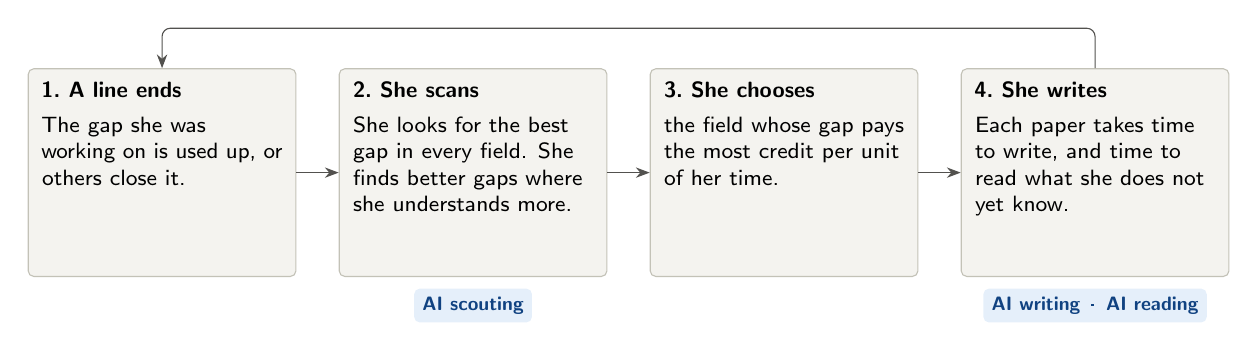
\begin{tikzpicture}[font=\sffamily\footnotesize,>={Stealth[length=5pt]},
  stepbox/.style={draw=axisc,fill=paperc,rounded corners=2pt,inner sep=5pt,anchor=north west},
  tag/.style={fill=hblue!12,text=hbluedark,rounded corners=2pt,inner sep=3pt,font=\sffamily\scriptsize\bfseries,anchor=north}]
\node[stepbox] (s1) at (0,0) {\stepcell{1.\ A line ends}{The gap she was working on is used up, or others close it.}};
\node[stepbox] (s2) at (1.555in,0) {\stepcell{2.\ She scans}{She looks for the best gap in every field. She finds better gaps where she understands more.}};
\node[stepbox] (s3) at (3.11in,0) {\stepcell{3.\ She chooses}{the field whose gap pays the most credit per unit of her time.}};
\node[stepbox] (s4) at (4.665in,0) {\stepcell{4.\ She writes}{Each paper takes time to write, and time to read what she does not yet know.}};
\draw[->,inktwo] (s1) -- (s2);
\draw[->,inktwo] (s2) -- (s3);
\draw[->,inktwo] (s3) -- (s4);
\draw[->,inktwo,rounded corners=3pt] (s4.north) -- ++(0,0.2in) -| (s1.north);
\node[tag] at ([yshift=-4pt]s2.south) {AI scouting};
\node[tag] at ([yshift=-4pt]s4.south) {AI writing\enspace\textperiodcentered\enspace AI reading};
\end{tikzpicture}
\caption{One round of a researcher's work, and where AI enters.}\label{fig:cycle}
\end{figure}

\subsection{Fields, homes and understanding}

There are $K$ fields, indexed by $k$. Time is continuous. A mass $N_j$ of researchers have field $j$ as their \emph{home}. Homes are fixed.

A researcher whose home is $j$ already knows a share $u_{jk}\in(0,1)$ of the literature behind a paper in field $k$. This is her \emph{understanding} of field $k$. She understands her own field best: $u_{jk}\le u_{jj}$ for every $k$. The matrix $(u_{jk})$ is the map of science: two fields are close when the researchers of one understand the other.

\subsection{What AI changes}

AI enters as three numbers. Each describes what a researcher can do with the tools she has.

\begin{center}\small
\begin{tabularx}{\textwidth}{@{}C{0.35in}P{1.05in}L@{}}
\toprule
 & Capability & Meaning \\
\midrule
$a$ & Writing speed & Papers a year she could write if she did nothing else. It covers everything between having a gap and having a paper: derivations, code, experiments, drafting. \\
$b$ & Reading speed & Papers a year she could absorb if she did nothing else. It rises when a tool summarises a literature for her or explains it to her. \\
$\alpha$ & Scouting & The share of what she does not understand about a field that AI makes up for when she looks for gaps there, $0\le\alpha<1$. It rises when a tool can find open questions and tell her whether a question is already answered. \\
\bottomrule
\end{tabularx}
\end{center}

With scouting $\alpha$ she looks for gaps in field $k$ as if her understanding were
\begin{equation}\label{eq:ut}
\ut_{jk} \;=\; u_{jk}+\alpha\,(1-u_{jk}).
\end{equation}
Scouting helps her find gaps. It does not spare her the reading: to write in field $k$ she must know its literature herself, and that takes time at speed $b$.

\subsection{Lines of work and the scan}

She works on one \emph{line} at a time. A line is a gap in some field, together with the papers she writes on it. A line ends at rate $\kappa$, whatever its field: the gap is used up, or others close it. She stays on a line until it ends.

When a line ends she \emph{scans} every field for the next one. In field $k$ the best gap she finds is worth
\begin{equation}\label{eq:gap}
q(\ut_{jk})\,Z_k \qquad\text{units of credit per paper.}
\end{equation}
Credit is the value of a contribution as the profession scores it. Citations are its nearest measure. The two factors are these.
\begin{itemize}
\item $Z_k$ is the raw value of the best gap in field $k$. It is random, with $\Pr(Z_k\le z)=\exp(-G_k z^{-\theta})$ and $\theta>1$, independently across fields, scans and researchers. $G_k$ is the \emph{abundance of gaps} in field $k$. The parameter $\theta$ measures how alike gaps are: when it is large, the best gap in a field is seldom much better than a typical one.
\item $q(\ut_{jk})$ is her \emph{gap efficiency}: the share of that value she captures, given what she understands. A researcher who knows little of a field misses its best gaps, and cannot be sure that a gap she sees is still open. The function $q$ maps $(0,1]$ into $(0,1]$, is increasing and log-concave, and has $q(1)=1$. The leading case is $q(u)=u^{\sigma}$ with $\sigma>0$.
\end{itemize}
Appendix~\ref{app:scan} derives \eqref{eq:gap} from a model in which gaps arrive at random and she notices some of them.

\subsection{Time}

A paper in field $k$ builds on $m_k$ earlier papers, and she must know them to write it. She already knows a share $u_{jk}$ of them. She reads the rest,
\begin{equation}\label{eq:ell}
\ell_{jk}\;=\;m_k\,(1-u_{jk})\qquad\text{papers.}
\end{equation}
A paper in field $k$ therefore takes her
\begin{equation}\label{eq:tau}
\tau_{jk}\;=\;\frac1a+\frac{\ell_{jk}}{b}\qquad\text{years,}
\end{equation}
of which a share
\begin{equation}\label{eq:omega}
\omega_{jk}\;=\;\frac{1/a}{\tau_{jk}}\;=\;\frac{1}{1+(a/b)\,\ell_{jk}}
\end{equation}
is spent writing and the rest reading. We call $a/b$ the \emph{pace}: how fast she writes relative to how fast she reads.

Every paper has its own literature, and what she understands does not change. Her second paper in a field costs her as much reading as her first.

\subsection{The researcher's problem}

On a line in field $k$ she earns credit at the rate
\begin{equation}\label{eq:V}
V_{jk}\;=\;\frac{q(\ut_{jk})\,Z_k}{\tau_{jk}} .
\end{equation}
She maximises expected discounted credit. Every line lasts $1/\kappa$ on average wherever it is, so the choice of a line does not affect what comes after it. The best she can do at each scan is to take the field with the highest credit rate (Lemma~\ref{lem:choice} in Appendix~\ref{app:proofs}):
\begin{equation}\label{eq:choice}
k^{*}\;=\;\argmax_{k}\,V_{jk}.
\end{equation}
Write $\pi_{jk}$ for the probability that she takes a line in field $k$, and $W_j=\E\big[\max_k V_{jk}\big]$ for her expected credit per unit of time.

\subsection{Fields}

Let $P_k$ be the number of papers written in field $k$ per unit of time. Gaps are scarcer where more is being written:
\begin{equation}\label{eq:crowd}
G_k\;=\;A_k\,P_k^{-\eta},\qquad \eta\ge 0 .
\end{equation}
$A_k$ is the \emph{opportunity} in field $k$. It rises when a discovery, an instrument or a tool opens questions there. The parameter $\eta$ measures crowding. With $\eta=0$ fields do not interact.

\begin{defn}{Stationary equilibrium}{eq}
A stationary equilibrium is a vector of paper flows $P=(P_1,\dots,P_K)$, all positive, such that when gaps are given by \eqref{eq:crowd} and every researcher chooses by \eqref{eq:choice}, the papers written in each field add up to its flow:
\begin{equation}\label{eq:flow}
P_k\;=\;\sum_{j=1}^{K} N_j\,\frac{\pi_{jk}}{\tau_{jk}}\qquad\text{for every } k .
\end{equation}
\end{defn}

\begin{keybox}[The baseline in one place]
\small
\begin{tabularx}{\linewidth}{@{}P{0.95in}L@{}}
Given & $K$ fields; researchers $N_j$; understanding $u_{jk}$; literatures $m_k$; opportunities $A_k$; gap efficiency $q(\cdot)$; $\theta$ (how alike gaps are), $\eta$ (crowding), $\kappa$ (how soon a line ends). \\
AI & writing speed $a$, reading speed $b$, scouting $\alpha$. \\
Scan & best gap in field $k$ is worth $q\big(u_{jk}+\alpha(1-u_{jk})\big)Z_k$ a paper, $\Pr(Z_k\le z)=e^{-G_kz^{-\theta}}$. \\
Time & a paper takes $\tau_{jk}=1/a+m_k(1-u_{jk})/b$. \\
Choice & she takes the field with the highest $q(\ut_{jk})Z_k/\tau_{jk}$, and keeps it until the line ends. \\
Fields & $G_k=A_kP_k^{-\eta}$, and $P_k=\sum_jN_j\pi_{jk}/\tau_{jk}$. \\
Solved for & where she works $\pi_{jk}$, her credit $W_j$, papers $P_k$ and gaps $G_k$ in every field. \\
\end{tabularx}
\end{keybox}

\subsection{A worked example}\label{sec:example}

Table~\ref{tab:example} puts numbers on one researcher. She can write three papers a year ($a=3$) and read a hundred ($b=100$). A paper builds on forty others ($m_k=40$). She knows 90\% of the literature at home, 70\% in the two fields next door and 50\% in twenty fields far away. Gaps are equally abundant everywhere, $q(u)=u$, $\theta=4$ and $\alpha=0$. The numbers are chosen so that the split of her papers is close to the one on arXiv in 2022. They are an illustration, not an estimate.

\begin{table}[H]
\centering\small
\caption{A worked example.}\label{tab:example}
\begin{tabularx}{\textwidth}{@{}LC{0.72in}C{0.72in}C{0.72in}@{}}
\toprule
 & At home & Next door & Far away \\
\midrule
\tabinput{tables/example.tex}
\bottomrule
\end{tabularx}
\end{table}

At home she reads four papers for each one she writes, and writes 2.7 a year. Far away she reads twenty and writes 1.9. The last four rows are results, explained next.

% ------------------------------------------------------------------ 3
\section{What follows}\label{sec:results}

Propositions~\ref{prop:where} to~\ref{prop:worth} take the abundance of gaps $G=(G_1,\dots,G_K)$ as given. Proposition~\ref{prop:eq} closes the model. Throughout, $q_{jk}$ stands for $q(\ut_{jk})$. Proofs are in Appendix~\ref{app:proofs}.

\begin{prop}{Where she works}{where}
\begin{enumerate}[label=(\roman*),leftmargin=2em]
\item She takes a line in field $k$ with probability
\begin{equation}\label{eq:pi}
\pi_{jk}\;=\;\frac{G_k\,(q_{jk}/\tau_{jk})^{\theta}}{\Phi_j},\qquad \Phi_j\;=\;\sum_{l=1}^{K}G_l\,(q_{jl}/\tau_{jl})^{\theta}.
\end{equation}
This is also the share of her time that she spends in field $k$. The share of her papers that she writes in field $k$ is $s_{jk}=(\pi_{jk}/\tau_{jk})\big/\sum_l(\pi_{jl}/\tau_{jl})$.
\item Her expected credit per unit of time is
\begin{equation}\label{eq:W}
W_j\;=\;\Gamma\!\big(1-\tfrac1\theta\big)\,\Phi_j^{1/\theta},
\end{equation}
where $\Gamma$ is the gamma function.
\item Relative to home,
\begin{equation}\label{eq:gravity}
\frac{\pi_{jk}}{\pi_{jj}}\;=\;\frac{G_k}{G_j}\;d_{jk}^{-\theta},\qquad d_{jk}\;=\;\underbrace{\frac{\tau_{jk}}{\tau_{jj}}}_{\text{time penalty}}\times\underbrace{\frac{q_{jj}}{q_{jk}}}_{\text{scouting penalty}} .
\end{equation}
\end{enumerate}
\tcblower
\inwords Her work follows a gravity equation. A field attracts her in proportion to its gaps and repels her in proportion to its \emph{distance} $d_{jk}$ from her home. Distance is the product of two penalties: the extra time a paper takes her there, and the gaps she fails to find there. A raw gap away from home must be $d_{jk}$ times as good as the best one at home before she takes it: 1.56 times next door and 2.57 times far away in Table~\ref{tab:example}. The elasticity is $\theta$: when gaps are alike, small differences in distance move a lot of work.
\end{prop}

Readers who know the trade literature will recognise the structure of Eaton and Kortum (2002), with fields in place of countries and reading time in place of transport costs. It is also that of models of occupational choice in which talent is drawn from the same distribution (Hsieh, Hurst, Jones and Klenow 2019). This form is what gives closed forms for any number of fields and any map of science.

\begin{prop}{What going away costs}{cost}
\begin{enumerate}[label=(\roman*),leftmargin=2em]
\item On a line in field $k$ she writes $1/\tau_{jk}$ papers per unit of time.
\item The credit rate of the line she chooses has the same distribution whichever field it is in: $\Pr\big(V_{jk}\le v \,\big|\, k^{*}=k\big)=\exp(-\Phi_j v^{-\theta})$ for every $k$.
\item The expected credit of a paper on a line she chose in field $k$ is therefore $W_j\,\tau_{jk}$.
\end{enumerate}
\tcblower
\inwords Compare a line in a field where a paper takes her longer with a line at home. Away she writes fewer papers, $\tau_{jj}/\tau_{jk}$ as many. Each is worth more, $\tau_{jk}/\tau_{jj}$ as much on average. The two cancel exactly. She is less productive in papers and no less productive in credit, because she leaves home only for a gap that is good enough to pay for the reading. In Table~\ref{tab:example} she writes 30\% fewer papers a year on a line far away, and each is worth 43\% more.
\end{prop}

The exact cancellation in Proposition~\ref{prop:cost} comes from the form of the distribution of $Z_k$. With thinner tails, such as log-normal values, selection offsets only part of the cost of distance, and lines away from home pay less. The baseline is the case in which selection is strongest.

\begin{prop}{Deeper or wider}{dw}
Let field $k$ be farther from her than home: she must read more there, $\ell_{jk}>\ell_{jj}$, and she understands it less, $u_{jk}<u_{jj}$. Then $\omega_{jk}<\omega_{jj}$. Write $g_{jk}=\dfrac{q'(\ut_{jk})}{q(\ut_{jk})}\,(1-u_{jk})$ for what a little more scouting adds to $\ln q_{jk}$.
\begin{enumerate}[label=(\roman*),leftmargin=2em]
\item \emph{Faster writing sends her deeper:}
\[\frac{\partial\ln(\pi_{jk}/\pi_{jj})}{\partial\ln a}\;=\;-\,\theta\,(\omega_{jj}-\omega_{jk})\;<\;0 .\]
\item \emph{Faster reading sends her wider, by the same amount:}
\[\frac{\partial\ln(\pi_{jk}/\pi_{jj})}{\partial\ln b}\;=\;+\,\theta\,(\omega_{jj}-\omega_{jk})\;>\;0 .\]
Only the pace $a/b$ matters: if writing and reading speed rise in the same proportion, every $\pi_{jk}$ is unchanged.
\item \emph{Better scouting sends her wider:}
\[\frac{\partial\ln(\pi_{jk}/\pi_{jj})}{\partial\alpha}\;=\;\theta\,(g_{jk}-g_{jj})\;>\;0 .\]
\item The same holds for the shares of her papers, $s_{jk}/s_{jj}$, with $1+\theta$ in place of $\theta$ in (i) and~(ii).
\end{enumerate}
The time penalty $\tau_{jk}/\tau_{jj}$ rises with the pace, from $1$ when $a/b\to0$ to $\ell_{jk}/\ell_{jj}$ when $a/b\to\infty$.
\tcblower
\inwords A paper costs writing time, which is the same everywhere, and reading time, which is larger away from home. Faster writing shrinks the part that is the same everywhere, so the part that differs weighs more, and distance grows. Faster reading shrinks the part that differs. Scouting works on the other penalty, the gaps she fails to find.

There are two limits. If writing becomes free and reading does not, the time penalty reaches $\ell_{jk}/\ell_{jj}$: in the example 3 next door and 5 far away, against 1.2 and 1.4 today. AI that only writes builds walls between fields. If reading becomes free and scouting perfect, distance disappears and she goes wherever the gaps are, $\pi_{jk}=G_k/\sum_lG_l$, whatever her home. AI that reads and scouts takes the walls down.
\end{prop}

Table~\ref{tab:scen} and Figure~\ref{fig:mech} show the sizes in the worked example. Doubling writing speed alone raises the share of her papers written at home from 63\% to 80\%. Doubling reading speed alone lowers it to 47\%. Doubling both leaves it where it was.

\begin{table}[H]
\centering\small
\caption{What each capability does in the worked example (gaps given).}\label{tab:scen}
\begin{tabularx}{\textwidth}{@{}LC{0.52in}C{0.68in}C{0.62in}C{0.6in}C{0.52in}C{0.52in}@{}}
\toprule
 & \multicolumn{3}{c}{Share of her papers} & Papers & \multicolumn{2}{c}{Change in} \\
\cmidrule(lr){2-4}\cmidrule(l){6-7}
 & home & next door & far away & a year & papers & credit \\
\midrule
\tabinput{tables/scenarios.tex}
\bottomrule
\end{tabularx}
\end{table}

\begin{figure}[H]
\centering
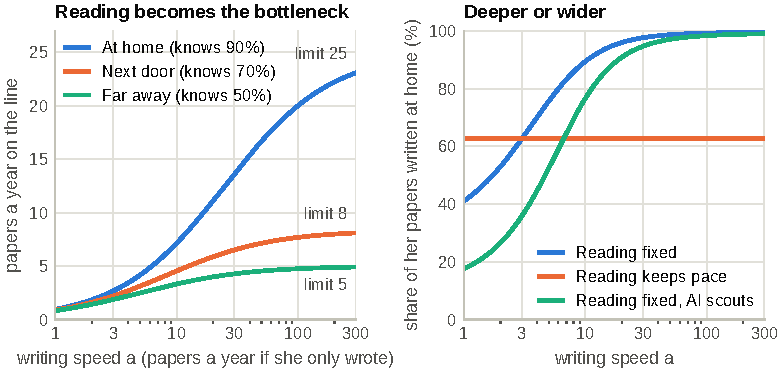
\includegraphics[width=\textwidth]{mechanism.pdf}
\caption{Left: papers a year on a line as writing gets faster, with reading speed fixed; each line approaches the limit $b/\ell_{jk}$. Right: the share of her papers written at home as writing gets faster, in three cases. Reading speed stays at its level in Table~\ref{tab:example}; it rises in step with writing speed; it stays fixed and AI scouts with $\alpha=\tfrac12$.}\label{fig:mech}
\end{figure}

\begin{prop}{What a capability is worth}{worth}
Let $\bar\omega_j=\sum_k\pi_{jk}\,\omega_{jk}$ be the share of all her time that she spends writing, and $R_j=\sum_k\pi_{jk}/\tau_{jk}$ the number of papers she writes per unit of time.
\begin{enumerate}[label=(\roman*),leftmargin=2em]
\item \emph{Credit.}\enspace $\displaystyle\frac{\partial\ln W_j}{\partial\ln a}=\bar\omega_j,\qquad \frac{\partial\ln W_j}{\partial\ln b}=1-\bar\omega_j,\qquad \frac{\partial\ln W_j}{\partial\alpha}=\sum_k\pi_{jk}\,g_{jk}.$
\item \emph{Papers.}\enspace With $\Var_j=\sum_k\pi_{jk}(\omega_{jk}-\bar\omega_j)^2$ and $\Cov_j=\sum_k\pi_{jk}(\omega_{jk}-\bar\omega_j)(g_{jk}-\bar g_j)$, where $\bar g_j=\sum_k\pi_{jk}g_{jk}$,
\[
\frac{\partial\ln R_j}{\partial\ln a}=\bar\omega_j+(1+\theta)\frac{\Var_j}{\bar\omega_j},\qquad
\frac{\partial\ln R_j}{\partial\ln b}=1-\bar\omega_j-(1+\theta)\frac{\Var_j}{\bar\omega_j},\qquad
\frac{\partial\ln R_j}{\partial\alpha}=\theta\,\frac{\Cov_j}{\bar\omega_j}.
\]
\item \emph{The bottleneck.}\enspace As $a\to\infty$ with $b$ fixed, she writes $b/\ell_{jk}$ papers per unit of time on a line in field $k$, and $W_j$ converges to a finite limit that is proportional to $b$.
\end{enumerate}
\tcblower
\inwords (i) A capability is worth the time it saves. In the worked example she spends 80\% of her time writing, so writing 1\% faster raises her credit by 0.8\% and reading 1\% faster by 0.2\%. Where she then chooses to work adds nothing to first order.

(ii) Papers and credit come apart. Faster writing raises her papers by more than her credit, because she moves home, where papers are quick. Faster reading raises her papers by less than her credit, and can lower them. Better scouting lowers her papers when the fields it opens are those where papers take longest ($\Cov_j<0$). In both cases she moves to work that takes longer and is worth more. In Table~\ref{tab:scen}, scouting cuts her papers by 9\% and raises her credit by 24\%.

(iii) Reading becomes the bottleneck. Once writing is fast, only reading speed raises output (Figure~\ref{fig:mech}, left).
\end{prop}

\begin{prop}{Equilibrium}{eq}
For every $\eta\ge0$:
\begin{enumerate}[label=(\roman*),leftmargin=2em]
\item A stationary equilibrium exists and is unique. It is the limit, from any positive starting point, of the iteration
\begin{equation}\label{eq:map}
P_k\;\longleftarrow\;\bigg[A_k\sum_{j}\frac{N_j\,q_{jk}^{\theta}\,\tau_{jk}^{-(1+\theta)}}{\sum_lA_lP_l^{-\eta}(q_{jl}/\tau_{jl})^{\theta}}\bigg]^{\frac{1}{1+\eta}}.
\end{equation}
\item \emph{Balanced progress.} If $a$ and $b$ are both multiplied by $\lambda>0$, every $P_k$ is multiplied by $\lambda$, every share $\pi_{jk}$ is unchanged, and every $W_j$ is multiplied by $\lambda^{1-\eta/\theta}$.
\item \emph{Balanced growth.} If every $N_j$ is multiplied by $\lambda>0$, every $P_k$ is multiplied by $\lambda$, every share $\pi_{jk}$ is unchanged, and every $W_j$ is multiplied by $\lambda^{-\eta/\theta}$.
\item \emph{Symmetric worlds.} Let the fields lie on a circle, with $N_j$, $A_k$ and $m_k$ equal across fields and $u_{jk}$ a function of the distance between $j$ and $k$ only. Then all $P_k$ are equal, $G$ drops out of \eqref{eq:pi}, and the responses in Propositions~\ref{prop:dw} and~\ref{prop:worth}(ii) hold in equilibrium as stated. Each elasticity of credit in Proposition~\ref{prop:worth}(i) is lower by $\eta/\theta$ times the matching elasticity of papers in~\ref{prop:worth}(ii).
\end{enumerate}
\tcblower
\inwords The model always has exactly one answer. The direction of research does not respond to progress that is balanced or to growth that is balanced. It responds to imbalance: a change in the pace, in scouting, in opportunities, or in the number of researchers in one field relative to the others. Crowding takes back part of the gain in credit: under balanced progress, the share $\eta/\theta$ of it.
\end{prop}

Two remarks. First, the proof also covers $-\tfrac12<\eta<0$, the case in which papers open more gaps than they close. Second, uneven growth moves work outwards. In the five-field example of the check script, doubling the researchers of one field lowers the share of their time spent at home from 83\% to 79\%. This is a numerical example, not a theorem. It is the counterpart here of the earlier draft's idea that more researchers and faster researchers are absorbed differently: more researchers in a field push its work outwards, faster writing pulls it home.

% ------------------------------------------------------------------ 4
\section{The model and the data}\label{sec:data}

\subsection{What measures what}

Each object of the baseline has a counterpart in data on papers, authors and dates. Table~\ref{tab:data} lists them with the first cuts from arXiv. In these cuts a field is an arXiv category, home is an author's most frequent category in the three previous years, and comparisons are matched, not causal (\texttt{docs/empirical\_design.md}).

\begin{table}[H]
\centering\small
\caption{Objects of the model and their counterparts.}\label{tab:data}
\begin{tabularx}{\textwidth}{@{}P{1.4in}P{2.2in}L@{}}
\toprule
In the model & What measures it & First cut \\
\midrule
Shares of her papers, $s_{jk}$ & An author's papers at home, in a neighbouring category, in another broad field & 60\%, 20\%, 20\% in 2022;\newline 51\%, 31\%, 18\% in 2026 \\
Time penalty, $\tau_{jk}/\tau_{jj}$ & Her output around a move, against matched authors who did not move & Without a local co-author, a near move costs 0.10 years of output and a far move 0.67 \\
Reading per paper, $\ell_{jk}$ & Her reference list: its length, and how much of it is new to her & First paper in a field: 6\% fewer references \\
Credit per paper & Citations & First paper in a field: 0.14 log points fewer \\
Writing speed, $a$ & Papers per author & 2.5 in January to September 2022, 3.4 in the same months of 2026 \\
Understanding, $u_{jk}$ & Overlap of two fields' reference lists; similarity of their texts & Not yet built \\
Gaps, $G_{k}$ & Destination-by-year effects in \eqref{eq:grav} & Not yet estimated \\
A line's length, $1/\kappa$ & Runs of an author's papers in one field & Not yet measured \\
\bottomrule
\end{tabularx}
\end{table}

\subsection{The estimating equation}

Let $X_{jk}=N_j\pi_{jk}/\tau_{jk}$ be the papers written in field $k$ by researchers whose home is $j$. By Proposition~\ref{prop:where},
\begin{equation}\label{eq:grav}
\ln X_{jk}\;=\;\underbrace{h_j}_{\text{home}}\;+\;\underbrace{\ln G_k}_{\text{destination}}\;\underbrace{-\,(1+\theta)\ln\!\big(1+\tfrac ab\,\ell_{jk}\big)+\theta\ln q\big(u_{jk}+\alpha(1-u_{jk})\big)}_{\text{distance}} ,
\end{equation}
where $h_j=\ln N_j-\ln\Phi_j+(1+\theta)\ln a$ collects what is specific to the home field.
With one such equation a year, home-by-year effects absorb everything specific to the home field, and destination-by-year effects absorb opportunities and crowding. What is left is how flows fall with distance, and how that changes over time. A rising pace makes the fall steeper. Cheaper understanding makes it flatter.

The two can be told apart. The pace also changes how many papers she writes on a line away from home relative to a line at home, $\tau_{jj}/\tau_{jk}$. Scouting does not. In the model a line in field $k$ costs her $(1/\kappa)(1-\tau_{jj}/\tau_{jk})$ years of home output, which is what the output cost of a move measures.

\subsection{What a counterfactual needs}

As in models of trade (Dekle, Eaton and Kortum 2008), the effect of a change in capabilities can be computed from a few observed shares. The levels of opportunities, of understanding and of the number of researchers are not needed. Write $\hat x=x'/x$ for the change in any $x$. For changes $\hat a$ and $\hat b$ and a new $\alpha'$,
\begin{gather*}
\hat\tau_{jk}=\frac{\omega_{jk}}{\hat a}+\frac{1-\omega_{jk}}{\hat b},\qquad
\hat q_{jk}=\frac{q\big(u_{jk}+\alpha'(1-u_{jk})\big)}{q\big(u_{jk}+\alpha(1-u_{jk})\big)},\\[3pt]
\pi'_{jk}=\frac{\pi_{jk}\,\hat P_k^{-\eta}\,(\hat q_{jk}/\hat\tau_{jk})^{\theta}}{\sum_l\pi_{jl}\,\hat P_l^{-\eta}\,(\hat q_{jl}/\hat\tau_{jl})^{\theta}},\qquad
\hat P_k=\sum_j\frac{X_{jk}}{P_k}\,\frac{\pi'_{jk}/\pi_{jk}}{\hat\tau_{jk}},\qquad
\hat W_j=\Big[\sum_l\pi_{jl}\,\hat P_l^{-\eta}\,(\hat q_{jl}/\hat\tau_{jl})^{\theta}\Big]^{1/\theta}.
\end{gather*}
A change in writing or reading speed needs four things: the shares $\pi_{jk}$ (from the shares of papers, since $\pi_{jk}\propto s_{jk}\tau_{jk}$), who writes each field's papers $X_{jk}/P_k$, the writing shares $\omega_{jk}$, and the two elasticities $\theta$ and $\eta$. A change in scouting needs $\hat q_{jk}$ as well.

\subsection{What the baseline says about the first cuts}

\begin{enumerate}[leftmargin=1.7em]
\item \textbf{Writing got faster.} Established authors posted 2.5 papers in January to September 2022 and 3.4 in the same months of 2026.
\item \textbf{On its own, that sends work home. Work went the other way.} The share of papers written at home fell from 60\% to 51\%. Papers per author rose by 22\% at home and by 77\% away, and faster away than at home in eight of ten broad fields.
\item \textbf{So something else moved by more.} In the baseline that is cheaper understanding ($b$ or $\alpha$), or opportunities shifting towards other fields ($A_k$). Shares alone cannot tell these apart. Equation \eqref{eq:grav} and the output cost of a move can.
\item \textbf{Where the work went differs by field.} In computer science the rise is next door: the share of papers in neighbouring categories went from 29\% to 45\%, while the far share fell from 15\% to 12\%. Outside computer science the rise is far away: the far share rose in eight of nine broad fields, and the near share was flat or fell. In the baseline every capability moves far fields by more than near ones, and in the worked example any change in capabilities that raises the near share relative to home raises the far share by more. So the pattern outside computer science is the one that cheaper understanding gives. The pattern inside it is not: it needs opportunities to shift towards neighbouring fields, as when AI becomes a subject in many of them. Opportunities in computer science may also be what pulls the other fields' far moves. The destination-by-year effects in \eqref{eq:grav} are there to tell.
\item \textbf{One first cut speaks against the baseline.} Proposition~\ref{prop:cost} says that a paper away from home is worth more than a paper at home. An author's first paper in a new field is cited less, by 0.14 log points, and the difference is gone after three to five papers. Thinner tails would shrink the premium of Proposition~\ref{prop:cost}, but would not make a penalty fade with experience. Understanding that grows with work would. It is the first thing to add.
\end{enumerate}

% ------------------------------------------------------------------ 5
\section{What the baseline leaves out}\label{sec:out}

In the order in which they seem worth adding.

\begin{enumerate}[leftmargin=1.7em]
\item \textbf{Understanding that grows with work.} Here $u_{jk}$ is fixed. If reading and writing in a field raise it, a move becomes an investment: the first papers away are worth less, later ones more, and home itself becomes a choice. This would account for the lower citations of first papers, and for the 59\% of moves made without a local co-author that are never repeated.
\item \textbf{Co-authors.} A co-author who is at home in field $k$ lends her understanding. On arXiv 62\% of first papers in a new field have one, and those moves cost no output. AI that reads and scouts may replace such a co-author. So far it has not: the share of away papers with a local co-author has stayed between 42\% and 44\% since 2022.
\item \textbf{Reading to keep up.} Here the literature behind a paper, $m_k$, does not depend on how much is being written. If it rises with the flow $P_k$, faster writing by everyone raises everyone's reading, at home too. This is the mechanism of the earlier draft.
\item \textbf{A one-off cost of entering a field.} Here reading is per paper. With a cost paid once per field, the length of a line matters: short lines favour home.
\item \textbf{Fields that are born and used up.} Here opportunities $A_k$ are given. Gaps that get harder as a field matures, papers that open new fields, and the frontier are all outside.
\item \textbf{Duplication and quality.} Two researchers can take the same gap, and a paper written fast may be worth less. Both matter for what faster writing does to the value of what is produced.
\item \textbf{Welfare.} Credit is what researchers maximise here. Whether it measures the value of their work, and whether crowding makes the equilibrium inefficient, are open.
\end{enumerate}

% ------------------------------------------------------------------ appendix
\appendix
\section{Proofs}\label{app:proofs}

Throughout, $c_{jk}=q_{jk}/\tau_{jk}$, so that $V_{jk}=c_{jk}Z_k$ and $\Phi_j=\sum_lG_lc_{jl}^{\theta}$.

\begin{lem}{The choice at a scan}{choice}
Let her discount the future at rate $r>0$. At each scan it is optimal to take the line with the highest credit rate, and her expected discounted credit at a scan is $W_j/r$.
\end{lem}

\proofof{Proof}
Let $U_j$ be her expected discounted credit at a scan. A line with credit rate $v$ lasts a time $T$ that is exponential with rate $\kappa$, so it is worth $\E\big[\int_0^Te^{-rt}v\,\dd t+e^{-rT}U_j\big]=\dfrac{v}{r+\kappa}+\dfrac{\kappa}{r+\kappa}U_j$. The second term does not depend on the line. She therefore takes the line with the highest $v$. Taking expectations, $U_j=\dfrac{W_j}{r+\kappa}+\dfrac{\kappa}{r+\kappa}U_j$, so $U_j=W_j/r$. As $r\to0$ the same rule maximises her long-run average credit, which is $W_j$.

\proofof{Proof of Proposition~\ref{prop:where}}
Since $\Pr(V_{jk}\le v)=\Pr(Z_k\le v/c_{jk})=\exp(-G_kc_{jk}^{\theta}v^{-\theta})$ and the $Z_k$ are independent, $\Pr(\max_kV_{jk}\le v)=\exp(-\Phi_jv^{-\theta})$. The joint probability that field $k$ is chosen and its credit rate is at most $v$ is
\begin{equation}\label{eq:joint}
\int_0^v\theta G_kc_{jk}^{\theta}x^{-\theta-1}\exp\!\big(-\Phi_jx^{-\theta}\big)\,\dd x\;=\;\frac{G_kc_{jk}^{\theta}}{\Phi_j}\,\exp\!\big(-\Phi_jv^{-\theta}\big).
\end{equation}
Letting $v\to\infty$ gives \eqref{eq:pi}. Lines are taken with probabilities $\pi_{jk}$ and last $1/\kappa$ on average in every field, so $\pi_{jk}$ is also the share of her time spent in field $k$. In that time she writes $1/\tau_{jk}$ papers per unit of time, which gives $s_{jk}$. The maximum has distribution $\exp(-\Phi_jv^{-\theta})$, whose mean is $\Gamma(1-1/\theta)\Phi_j^{1/\theta}$ for $\theta>1$: this is \eqref{eq:W}. Dividing $\pi_{jk}$ by $\pi_{jj}$ gives \eqref{eq:gravity}.

\proofof{Proof of Proposition~\ref{prop:cost}}
Part (i) is \eqref{eq:tau}. Dividing \eqref{eq:joint} by $\pi_{jk}$ gives (ii). A paper on a line in field $k$ with credit rate $v$ earns $v\,\tau_{jk}$, and by (ii) the mean of $v$ on a chosen line is $W_j$ in every field: this is (iii).

\proofof{Proof of Proposition~\ref{prop:dw}}
From \eqref{eq:omega}, $\omega_{jk}$ falls with $\ell_{jk}$, so $\ell_{jk}>\ell_{jj}$ gives $\omega_{jk}<\omega_{jj}$. From \eqref{eq:gravity},
\[
\ln\frac{\pi_{jk}}{\pi_{jj}}=\ln\frac{G_k}{G_j}+\theta\big[\ln q(\ut_{jk})-\ln q(\ut_{jj})\big]-\theta\big[\ln\tau_{jk}-\ln\tau_{jj}\big].
\]
By \eqref{eq:tau}, $\partial\ln\tau_{jk}/\partial\ln a=-\omega_{jk}$ and $\partial\ln\tau_{jk}/\partial\ln b=-(1-\omega_{jk})$, which give (i) and~(ii). Multiplying $a$ and $b$ by the same number divides every $\tau_{jk}$ by it and leaves $q_{jk}$ unchanged, so $\Phi_j$ and every numerator in \eqref{eq:pi} change in the same proportion. For (iii), $\partial\ln q(\ut_{jk})/\partial\alpha=g_{jk}$ by \eqref{eq:ut}. Since $q$ is log-concave, $q'/q$ is decreasing; since $u_{jk}<u_{jj}$ and $\alpha<1$, $\ut_{jk}<\ut_{jj}$. So $q'(\ut_{jk})/q(\ut_{jk})\ge q'(\ut_{jj})/q(\ut_{jj})>0$ and $1-u_{jk}>1-u_{jj}$, hence $g_{jk}>g_{jj}$. For (iv), $s_{jk}/s_{jj}=(\pi_{jk}/\pi_{jj})(\tau_{jj}/\tau_{jk})$, which adds one more term in $\ln\tau_{jk}-\ln\tau_{jj}$. Last, $\tau_{jk}/\tau_{jj}=\big(1+\tfrac ab\ell_{jk}\big)\big/\big(1+\tfrac ab\ell_{jj}\big)$, which is increasing in $a/b$ when $\ell_{jk}>\ell_{jj}$, with the limits stated.

\proofof{Proof of Proposition~\ref{prop:worth}}
(i) By \eqref{eq:W}, $\ln W_j=\text{constant}+\tfrac1\theta\ln\Phi_j$, and $\partial\ln\Phi_j/\partial\ln a=\sum_k\pi_{jk}\,\theta\,\omega_{jk}$. The other two derivatives follow in the same way. (ii) From \eqref{eq:pi}, $\partial\ln\pi_{jk}/\partial\ln a=\theta(\omega_{jk}-\bar\omega_j)$. The share of her papers written in field $k$ is $s_{jk}=\pi_{jk}\omega_{jk}/\bar\omega_j$, because $1/\tau_{jk}=a\,\omega_{jk}$. So
\[
\frac{\partial\ln R_j}{\partial\ln a}=\sum_ks_{jk}\big[\theta(\omega_{jk}-\bar\omega_j)+\omega_{jk}\big]=(1+\theta)\sum_ks_{jk}\omega_{jk}-\theta\bar\omega_j=\bar\omega_j+(1+\theta)\frac{\Var_j}{\bar\omega_j},
\]
using $\sum_ks_{jk}\omega_{jk}=\bar\omega_j+\Var_j/\bar\omega_j$. The derivative with respect to $\ln b$ follows because $R_j$ is homogeneous of degree one in $(a,b)$. For scouting, $\tau_{jk}$ does not depend on $\alpha$ and $\partial\ln\pi_{jk}/\partial\alpha=\theta(g_{jk}-\bar g_j)$, so $\partial\ln R_j/\partial\alpha=\theta\sum_ks_{jk}(g_{jk}-\bar g_j)=\theta\,\Cov_j/\bar\omega_j$. (iii) As $a\to\infty$, $\tau_{jk}\to\ell_{jk}/b$ and $W_j\to b\,\Gamma(1-\tfrac1\theta)\big[\sum_kG_k(q_{jk}/\ell_{jk})^{\theta}\big]^{1/\theta}$.

\proofof{Proof of Proposition~\ref{prop:eq}}
(i) Substituting \eqref{eq:pi} and \eqref{eq:crowd} into \eqref{eq:flow} and collecting $P_k$ on the left gives $P_k^{1+\eta}=A_k\sum_jN_jq_{jk}^{\theta}\tau_{jk}^{-(1+\theta)}/\Phi_j(P)$, with $\Phi_j(P)=\sum_lA_lP_l^{-\eta}c_{jl}^{\theta}$. An equilibrium is a fixed point of the map $\Psi$ on the right of \eqref{eq:map}. $\Psi$ maps positive vectors to positive vectors. For $\eta\ge0$ each $\Phi_j$ is decreasing in $P$ and homogeneous of degree $-\eta$, so $\Psi$ is increasing and homogeneous of degree $\mu=\eta/(1+\eta)<1$. Measure the distance between two positive vectors by $D(P,P')=\max_k|\ln P_k-\ln P'_k|$ (Thompson's metric). If $D(P,P')=t$ then $e^{-t}P'\le P\le e^{t}P'$, so $e^{-\mu t}\Psi(P')\le\Psi(P)\le e^{\mu t}\Psi(P')$, that is, $D(\Psi(P),\Psi(P'))\le\mu\,D(P,P')$. The positive vectors with this distance are a complete metric space, since taking logarithms maps them onto $\R^K$ with the maximum norm. By the contraction mapping theorem $\Psi$ has exactly one fixed point, and the iteration converges to it from any starting point. For $-\tfrac12<\eta<0$, $\Psi$ is decreasing and homogeneous of degree $\mu\in(-1,0)$, and the same argument gives $D(\Psi(P),\Psi(P'))\le|\mu|\,D(P,P')$.

(ii) Let $P$ be the equilibrium, and multiply $a$ and $b$ by $\lambda$. Every $\tau_{jk}$ is divided by $\lambda$. At $\lambda P$ every $G_k$ is multiplied by $\lambda^{-\eta}$ and every $c_{jk}^{\theta}$ by $\lambda^{\theta}$, so the shares \eqref{eq:pi} are unchanged, and the right side of \eqref{eq:flow} is multiplied by $\lambda$. So $\lambda P$ is the equilibrium, and $\Phi_j$ is multiplied by $\lambda^{\theta-\eta}$. (iii) is the same argument with $\tau_{jk}$ unchanged. (iv) Rotating the labels of the fields maps an equilibrium into an equilibrium. By uniqueness the equilibrium is unchanged by rotation, so all $P_k$ are equal, all $G_k$ are equal, and $G$ cancels from \eqref{eq:pi}. Then $R_j$ does not depend on $G$, $P_k=N R_j$, and $\ln W_j=\text{constant}-\tfrac{\eta}{\theta}\ln R_j+\tfrac1\theta\ln\sum_kc_{jk}^{\theta}$, which gives the last statement.

\section{The scan from first principles}\label{app:scan}

Suppose that when she scans field $k$ the gaps open there are the points of a Poisson process: the number of gaps whose raw value exceeds $z$ is Poisson with mean $G_kz^{-\theta}$. $G_k$ is then the expected number of open gaps worth more than one unit of credit. She notices each gap independently with probability $\ut_{jk}^{\,\varsigma}$, $\varsigma>0$: the more she understands, the fewer she misses. The gaps she notices are again Poisson, with mean $\ut_{jk}^{\,\varsigma}G_kz^{-\theta}$ above $z$. The best gap she notices is below $z$ when she notices none above $z$, which has probability $\exp(-\ut_{jk}^{\,\varsigma}G_kz^{-\theta})$. It is therefore distributed as $\ut_{jk}^{\,\varsigma/\theta}Z_k$, with $Z_k$ as in Section~\ref{sec:model}.

Of the raw value of a gap she takes, she realises a share $\chi(\ut_{jk})$: with partial understanding she sometimes works on a question that is already answered, or misses what would make her answer matter. Together,
\[
q(\ut)\;=\;\ut^{\,\varsigma/\theta}\,\chi(\ut),
\]
which is increasing and log-concave when $\chi$ is, with $q(1)=1$ when $\chi(1)=1$. The leading case $q(u)=u^{\sigma}$ has $\chi(u)=u^{\sigma-\varsigma/\theta}$, with $\sigma\ge\varsigma/\theta$.

\section{Notation}\label{app:notation}

{\small
\begin{tabularx}{\textwidth}{@{}P{0.5in}P{2.05in}@{\hspace{16pt}}P{0.62in}L@{}}
\toprule
\multicolumn{2}{@{}l}{\sffamily\bfseries Given} & \multicolumn{2}{l}{\sffamily\bfseries Derived} \\
\midrule
$j$, $k$ & home field; field of work & $\ut_{jk}$ & understanding when scouting, \eqref{eq:ut} \\
$K$ & number of fields & $\ell_{jk}$ & papers to read for one paper, \eqref{eq:ell} \\
$N_j$ & researchers at home in $j$ & $\tau_{jk}$ & time per paper, \eqref{eq:tau} \\
$u_{jk}$ & understanding of field $k$ & $\omega_{jk}$ & writing share of that time, \eqref{eq:omega} \\
$m_k$ & literature behind a paper in $k$ & $Z_k$ & raw value of the best gap in $k$ \\
$A_k$ & opportunity in field $k$ & $G_k$ & abundance of gaps, \eqref{eq:crowd} \\
$q(\cdot)$ & gap efficiency & $V_{jk}$ & credit rate on a line in $k$, \eqref{eq:V} \\
$\theta$ & how alike gaps are & $\pi_{jk}$, $s_{jk}$ & her shares of time; of papers \\
$\eta$ & crowding & $\Phi_j$, $W_j$ & \eqref{eq:pi}; expected credit rate, \eqref{eq:W} \\
$\kappa$ & rate at which a line ends & $d_{jk}$ & distance, \eqref{eq:gravity} \\
$a$ & writing speed & $g_{jk}$ & gain from scouting, Proposition~\ref{prop:dw} \\
$b$ & reading speed & $\bar\omega_j$, $R_j$ & writing share; papers per unit of time \\
$\alpha$ & scouting & $P_k$, $X_{jk}$ & papers in field $k$; those by home $j$ \\
\bottomrule
\end{tabularx}
}

\end{document}
